

\subsection{Predicting Reactions with Labeled Topics}

[Boydstun et. al, 2013] labels each phrase in the October 4th, 2012 debate corpus with a topic ID. Each ID corresponds to a significant topic in the debate, such as "Defense" or "Labor, Employment, and Immigration." Unlike the topics found by LDA, these are hand-selected, with a single topic per phrase instead of a distribution over topics.

We are interested in whether using these hand-labeled topics, as opposed to the topics discovered using LDA, will improve or worsen performance predicting users' reactions to the debate.

Since we are working at the turn level, not the phrase level, we assimilate all topic IDs within a turn into a distribution over topics for that turn.

As before, each labeled topic present in the corpus is a feature. For a given turn, the value of that feature is the fraction of phrases within the turn labeled with that topic.

Once again we evaluate classification accuracy on three tasks, or labels: Whether a turn generates more or less than the median number of reactions per second, whether a turn generates more 'agree' or 'disagree' reactions, and whether a turn generates more or less than the median number of spin or dodge reactions per second.

Classification is done with Mallet, using Decision Tree, Maximum Entropy, and Naive Bayes classifiers. We perform 10-fold cross-validation using the 197 turns to calculate test accuracy and standard deviation:

\begin{table}[H]
\begin{centering}
\begin{tabular}{ l | l | l }
Classifier & Obama voters & Romney voters \\
\hline
DecTree & \textbf{0.695} (.131) &  \textbf{.719} (.150) \\
MaxEnt & \textbf{0.498} (.146) &  \textbf{.386} (.129) \\
Naive & \textbf{0.454} (.142) &  \textbf{.386} (.130) \\
\end{tabular}
\caption{Task 1 Accuracy and StdDev}
\end{centering}
\end{table}

\begin{table}[H]
\begin{centering}
\begin{tabular}{ l | l | l }
Classifier & Obama voters & Romney voters \\
\hline
DecTree & \textbf{0.519} (.095) &  \textbf{.455} (.090) \\
MaxEnt & \textbf{0.577} (.092) &  \textbf{.562} (.141) \\
Naive & \textbf{0.589} (.093) &  \textbf{.567} (.144) \\
\end{tabular}
\caption{Task 2 Accuracy and StdDev}
\end{centering}
\end{table}

\begin{table}[H]
\begin{centering}
\begin{tabular}{ l | l | l }
Classifier & Obama voters & Romney voters \\
\hline
DecTree & \textbf{0.803} (.106) &  \textbf{.805} (.150) \\
MaxEnt & \textbf{0.823} (.122) &  \textbf{.813} (.154) \\
Naive & \textbf{0.823} (.122) &  \textbf{.813} (.154) \\
\end{tabular}
\caption{Task 3 Accuracy and StdDev}
\label{tab:task3boydstun}
\end{centering}
\end{table}

For each classification task, we also keep track of the features that the Mallet Decision Tree learner selects most frequently for having the highest information gain. We can then look up the corresponding topics for the most valuable features.

\begin{table*}[H]
\begin{centering}
\begin{tabular}{| l | l | l |}
\hline
  & Best feature (Obama) & Best Feature (Romney) \\
\hline
Task 1 & labor/employment/immigration & government operations \\
	    & education & macroeconomics \\
	    & health & education \\
	    \hline
Task 2 & labor/employment/immigration & labor/employment/immigration \\
	    & government operations & education \\
	    & social welfare & macroeconomics  \\
	    \hline
Task 3 & candidate personal information & health \\
	    & social welfare & government operations \\
	    & labor/employment/immigration & candidate personal information \\
	    \hline
\end{tabular}
\caption{3 Features with highest information gain}
\end{centering}
\end{table*}


\subsection{User Reactions}

In the previous sections, we predict reactions to a turn based on the topics present in the turn. We find that we can do this reasonably well for some types of prediction, and also learn what topics contribute most certain reactions.

We can also ask what topics cause an individual user to react, rather than users in general. The label for prediction then becomes that user's reaction, and the features become the topics present in the discussion at the time of the reaction.

However, since we are now working at the individual level, we can also use features based on a user's responses to the ReactLabs survey questions, which we will call "user features." These include questions such as gender and political party, and also questions that ask the user to indicate agreement with one party or another on specific issues with a value between 0 and 100.

We are primarily interested in 1.) how well we can predict user reactions given user features and topic features, and 2.) how much topic features contribute to classification accuracy. Topic features are determined based on the turn in which the reaction occurs. We use features derived from both LDA topics and the Boydstun labeled topics. Labels are the 12 possible user reactions ("$Obama|Romney|Moderator : Agree|Disagree|Spin|Dodge$"). We use 10,000 reactions for 10-fold cross-validation.

\begin{table*}[H]
\begin{centering}
\begin{tabular}{ l | l | l | l }
Classifier & User features only & User + LDA & User + Boydstun \\
\hline
Decision Tree & \textbf{0.389} (.018) & \textbf{0.397} (.016) &  \textbf{.388} (.014) \\
Maximum Entropy & \textbf{.452} (.019) & \textbf{0.517} (.012) &  \textbf{.508} (.022) \\
Naive Bayes & \textbf{.443} (.020) & \textbf{0.481} (.012) &  \textbf{.460} (.013) \\
\end{tabular}
\caption{User reaction classification: accuracy and standard deviation}
\end{centering}
\end{table*}

We also plot confusion matrices using the best-performing classifier for both user features alone and user features combined with topic features.

\begin{figure}[H]
	\centering
	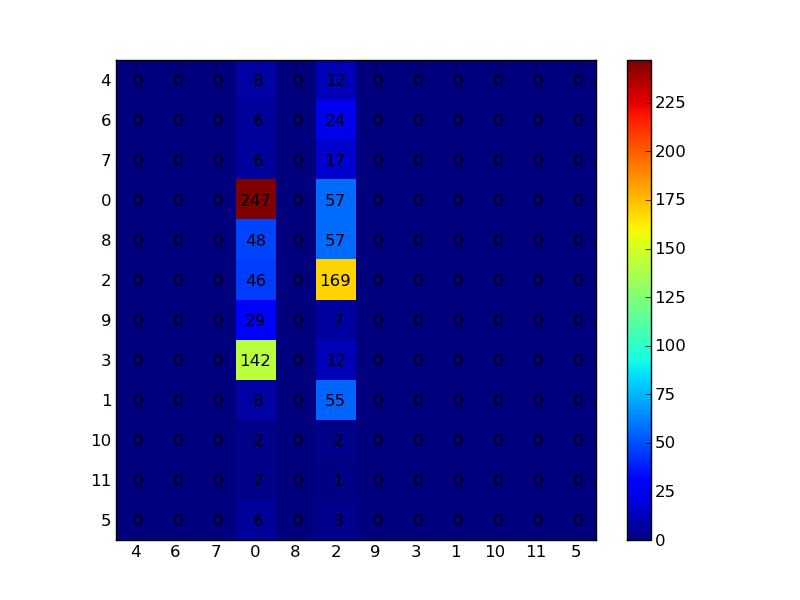
\includegraphics[scale=0.35]{Figures/no_topic_features_confusion.png}
	\caption{Confusion Matrix: Classification with user features only}
	\label{fig:useronlyconfusion}
\end{figure}

\begin{figure}[H]
	\centering
	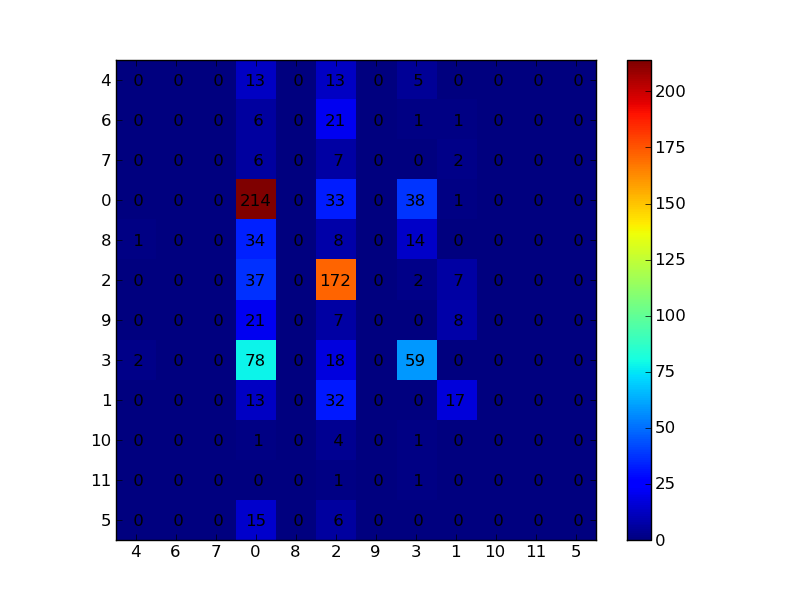
\includegraphics[scale=0.35]{Figures/boydstun_confusion.png}
	\caption{Confusion Matrix: Classification with user and topic features}
	\label{fig:boydstunconfusion}
\end{figure}


\begin{table}[H]
\begin{centering}
\begin{tabular}{ l | l | l | l }
 Code & Topic & Code & Topic \\
\hline
4 & Moderator:Agree & 9 & Romney:Dodge \\
6 & Obama:Spin & 3 & Romney:Disagree \\
7 & Obama:Dodge & 1 & Obama:Disagree \\
0 & Obama:Agree & 10 & Moderator:Spin \\
8 & Romney:Spin & 11 & Moderator:Dodge \\
2 & Romney:Agree & 5 & Moderator:Disagree \\

\end{tabular}
\caption{Topic code key}
\end{centering}
\end{table}
